% \clearpage

\section{NCBI Database}

The most important source of new data for GenBank is direct submissions from
scientists. GenBank depends on its contributors to help keep the database as
comprehensive, current, and accurate as possible. NCBI provides timely and accurate
processing and biological review of new entries, updates existing entries,
assists authors with submission of new data.

\section{NCBI Submission Submission Tool}
Thi NCBi data submission tool facilitates the creation of a Genbank ready for
submission.
The tool combines a reference genome (fasta file), the gene coordinates (gff
file) and the functional annotations of Blast2GO, creating a feature table
which will be validated with the tbl2asn program.
The `tbl2asn' command-line program is used to  automate the creation of
sequence records (.sqn files).
For more information about  tbl2asn visit:
\myurl{http://www.ncbi.nlm.nih.gov/genbank/tbl2asn2/ }.

When fisrt executed, the App will download the NCBI program
'tbl2asn' for your operating system allowing execution on Win, Mac and
Linux.
\par\textit{Note}: This tool requires an internet connection to download and
execute the tbl2asn program and to execute it, as it requieres a conection to
the NBI databases in order to validate the annotations.

\begin{figure}[!h] \centering
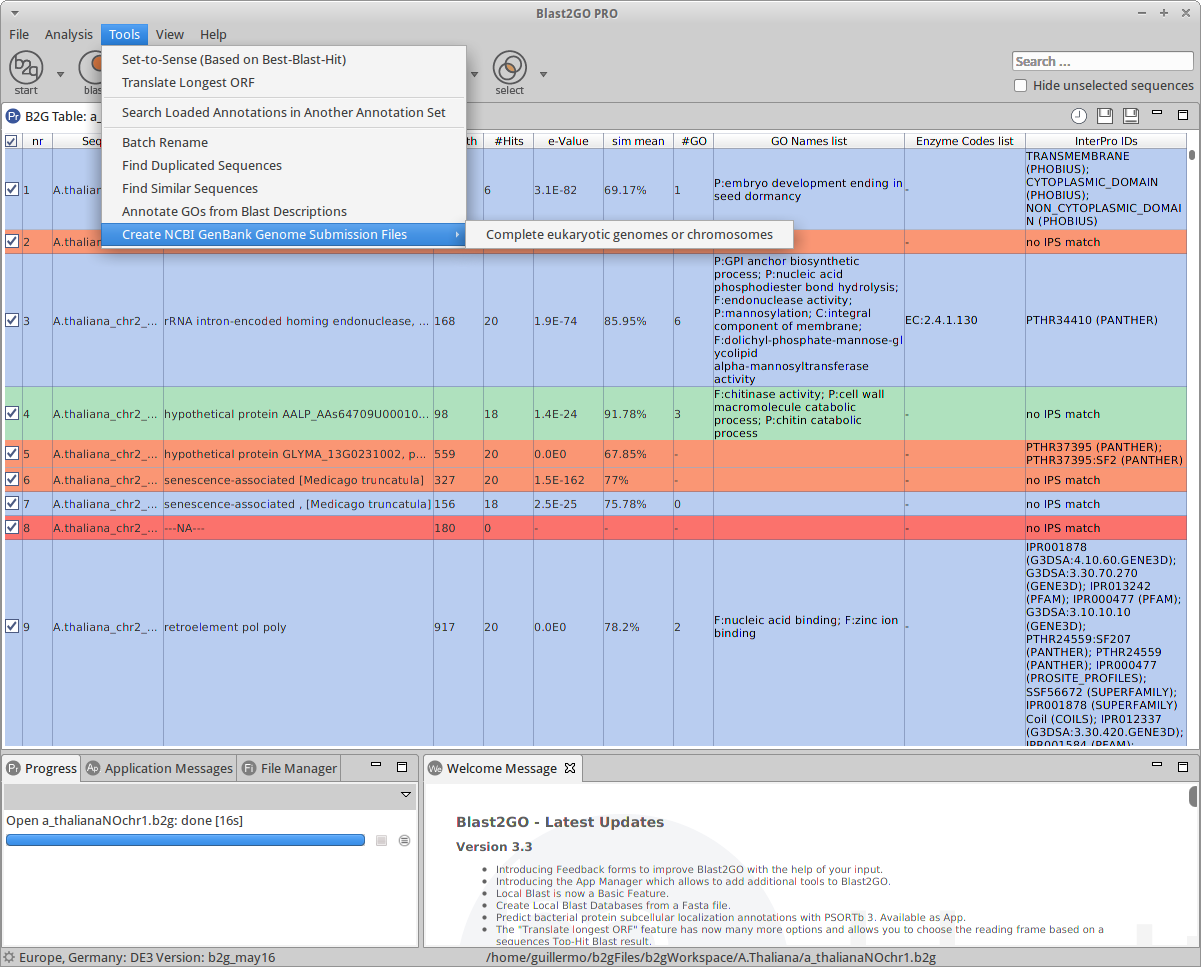
\includegraphics[width=100mm,scale=0.9]{img/Blast2GOPROmaimmenu.png}
\caption{NCBI Submission Tool}
\label{fig:ncbisubtool}
\end{figure}

\section{General Workflow}
To succesfully submit the annotated sequences, it is first necessary to prepare
the source of the annotations, i.e. the reference genome to
which the sequences belong, the position on the genome, and the functional
annotation. These files are processed by Blast2GO and validated by `tbl2asn'
program to create the ASN1 file (.sqn) and the validation files.

\begin{figure}[!h] \centering

\includegraphics[width=\textwidth]{img/Submission_workFlow.png}
\caption{General Workflow}
\label{fig:ncbisubworkflow}
\end{figure}
\newpage
\subsection{Input Files}
Three elements are necessaty to create the submission files:

\begin{itemize}
  \item \textbf{Reference genome}: This file provides the foundational
  nucleotide sequence and may contain one or more chromosomes The chromosome
  names in the fasta description line have to match the GFF file name.
  \item \textbf{Genomic annotation}: This data is provide by the GFF3 files, and
  is also used to link the Blast2GO annotations and the
  genome reference sequences in the Fasta file. A GFF3 is necessary for each
  chromosome, with the file name matching the chromosome name as it appears in
  the fasta file. The sequences name used in the Blast2GO project should appear
  in the feature column in the GFF3 file. The corresponding feature ID can be
  specified as parameter (default is seqName).
  \item \textbf{Functional annotation}: This information is provided by your
  Blast2GO project, and is intended to provide the functional features of your
  sequences, including gene names, Gene Ontology terms and enzyme numbers. The
  option to create the submission file is only activated when a Blast2GO
  Project file is loaded and selected.
  The sequence name of the functional annotation in your Blast2GO project has to
  match with a feature of your choice in the gff file.
\end{itemize}

\subsubsection{Preparing your data}

In order to integrate all the information and create the NCBI submission
files, we need to create informative links between them. As discussed above, the
GFF3 files act as a link between the genome sequence and the functional
annotation.

The FASTA, or multi-FASTA file may contain one or more chromosomes. The
chromosome names in the fasta description line have to match the GFF3 name,
additionally, the sequence name used in the Blast2GO project should appear in
the feature column in the GFF3 file. The corresponding feature ID can be specified
as a parameter (for the GFF files created by Augustus and Glimmer included in
Blast2GO, the IDs correspond to `seqName').


\begin{figure}[!h] \centering
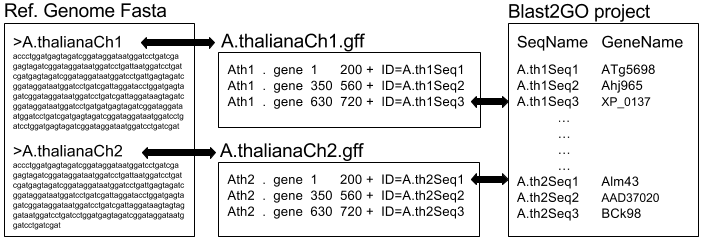
\includegraphics[width=\textwidth]{img/Submission_links.png}
\caption{Information integration schema}
\label{fig:ncbisublinkfiles}
\end{figure}


\section{Wizard pages}
\subsection {Page 1: Project Details}
\begin{itemize}
  \item \textbf{Locus tag}: The `locus tag' is an alfanumeric
  identifier of your project provided by the NCBI or user determined
  at the moment of the BioProject registration at:
  \myurl{https://submit.ncbi.nlm.nih.gov/subs/bioproject/}.
  \item \textbf{Laboratory ID}: The laboratory ID is a unique tag that refers to
  your own laboratory and allows the sequences to be associated with it.
  \item \textbf{Submission type}: Here you can choose the type of submission
  you want to perform.
  \begin{itemize}
    \item One or a few nucleotide sequences: use this option if you have a small
    dataset containing few sequences (less than a cromosome, or a
    chromosome on scaffold stage).
    \item Complete eukaryotic genomes or chromosomes: use this option if you have a
     complete data set without N's, conforming a chromosome or a whole genome.
    \item Incomplete genomes (WGS):  use this option if your dataset consist of
    incomplete genomic or chromosomal assemblies derived from shotgun sequencing
    methods.
    \end{itemize}
  \item \textbf{Assembly details (only for WGS submission)}: These details provide
  information about the more technical steps of the assembly.
  Here we can find:
	\begin{itemize}
 		\item Assembly method: The program or algorithms used assemble the genome.
 		\item Assembly name: This is a short project identifier.
 		\item Long assembly name: This is a larger and more explanatory name of your
 		project.
 		\item Genome coverage: This is the mean genome coverage obtained by the
 		assembler, and has a general format of one or more digits followed by an `x'
 		(e.g: 12x or 76x).
 		\item Sequencing technology: The name of the technology used to perform the
 		sequencing of the query genome. If the technology used is not in the list
 		shown, you can manually enter the name.
	\end{itemize}
  \item \textbf{Optional source qualifiers}: These are addtional sequence
  qualifiers to your all project, specifications of ooptional qualifiers allows
  you to add useful information regarding the organism chromosome, type, etc.
  If you are going to submit a WGS project,add the source information as
  organism and the relevant strain, breed, cultivar or isolate, if exists
  for the sequenced organism.
  \textit{Note: the `gcode' corresponding to the genetic code is only mandatory
  if the submitting organism is not specified or is not in the  NCBI Taxonomy Browser.}
\end{itemize}


\subsection {Page 2: Sequence Data and Annotation Files}
\begin{itemize}
 \item \textbf{Output Directory}: The creation and validation of the submitting
 sequences will produce multiple files that may be checked. This option allows
 the files to be saved in an existing folder, or to create a new one.

 \item \textbf{Fasta File}: The reference genome is the FASTA or multi-FASTA
 file containing the sequences to be submitted. This tool is designed to submit
 complete eukaryotic genomes or chromosomes. If you are submitting a single
 complete chromosome it must be in a single fasta entry, however, if you are
 submitting a complete genome, you must have a single entry for each chromosome.
 \textbf{Important note}: if this is a complete genome or chromosome submission,
  remove all the `Ns' present in the fasta file.

 \item \textbf{Genome annotation}:The genome annotation refers to the .gff file
 containing the gene coordinates for each annotated gene. This file must be
 named according to the dasta entry to which it corresponds.

 \item \textbf{Feature ID}: The feature ID of annotation refers to the flag on
 the ninth column of the gff file, which contains the name of the sequence,
 displayed as SeqName in Blast2GO.

 \item \textbf{Gene names}:  Here you can choose how to assign the names for
 your annotated sequences, the options are: ``hypothetical protein'', the
 ``SeqName'' assigned in the Blast2GO project or assign the name of the ``Top
 BLAST Hit''.
 If this last option is selected, you can set the threshold for:
 \begin{itemize}
   \item \textbf{E-value}:The minimum E-value obtained in the BLAST between the
   top BLAST hit and your query (default value is 1E-6).
   \item \textbf{Similaity}:The minimum percent similarity between the two
   sequences (0-100).
   \item \textbf{Coverage}:The minimum percent coverage between the two
   sequences (0-100).
\end{itemize}
\textbf{Important note}: If the threshold is not reached, the name of the gene
will be ``hypothetical protein''.
\end{itemize}
\textit{Note: all manual gene names annotations has higher priority.}

\begin{figure}
\centering
\begin{minipage}{.5\textwidth}
  \centering
  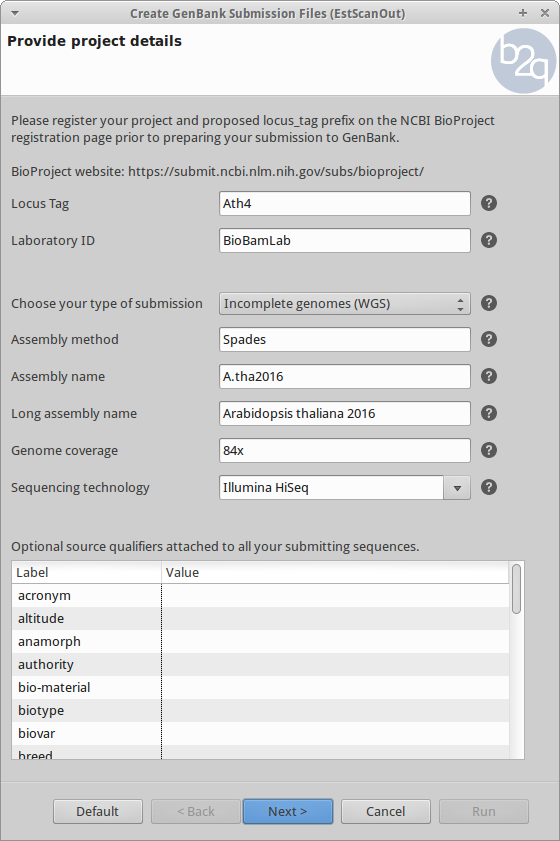
\includegraphics[width=0.8\linewidth]{img/WizardPage1.png}
  \caption{Project Details page}
  \label{fig:test1}
\end{minipage}%
\begin{minipage}{.5\textwidth}
  \centering
  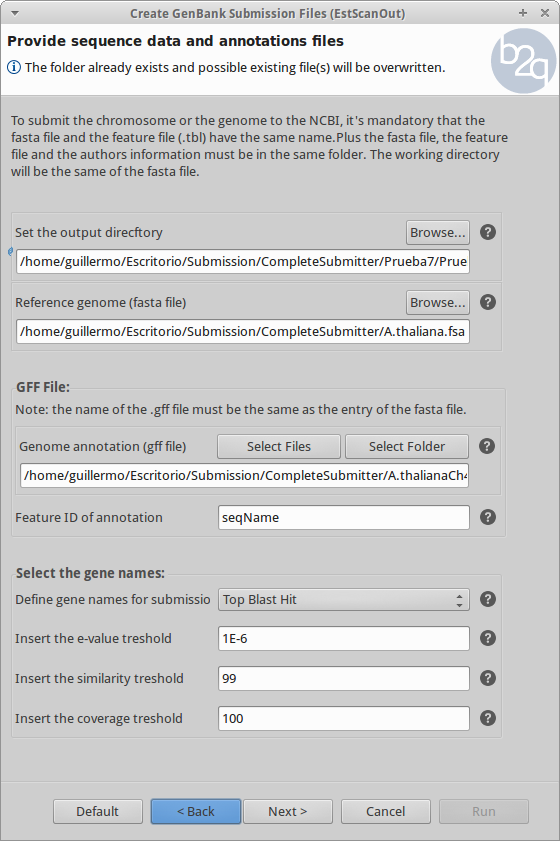
\includegraphics[width=0.8\linewidth]{img/WizardPage2.png}
 \caption{Sequence Data and Annotation Files page}
  \label{fig:test2}
\end{minipage}
\end{figure}

\newpage
\subsection {Page 3: Author's and Affiliation data}
\begin{itemize}
  \item \textbf{Contact data}: This page allows provison of the contact details
  for the submitting person. This information will not be publically visible,
  and only can be used by the NCBI staff for validation.
  \item \textbf{Institution data}: Information about the institution where the
  sequencing was performed is provided here.
  \item \textbf{Title of the manuscript}: This title is provisional and can be
  modified at any time via email request to the NCBI.
  \item \textbf{Release date}: This is the date when your submited and validated
  data will be accesible in the NCBI database. If the release date is The same
  day or before the submission, it will be automaticaly available once the data
  is validated.
  \item \textbf{Names and Initials}: Insert the names and initials of the
  individuals who must receive scientific credit for the generation of the
  sequences and annotations in this submission. If the authors are part of a
  consortium, it is not necessary that they appear as individual authors, as
  they are represented in the `Consortium' option.
\end{itemize}



\begin{figure}[!h] \centering
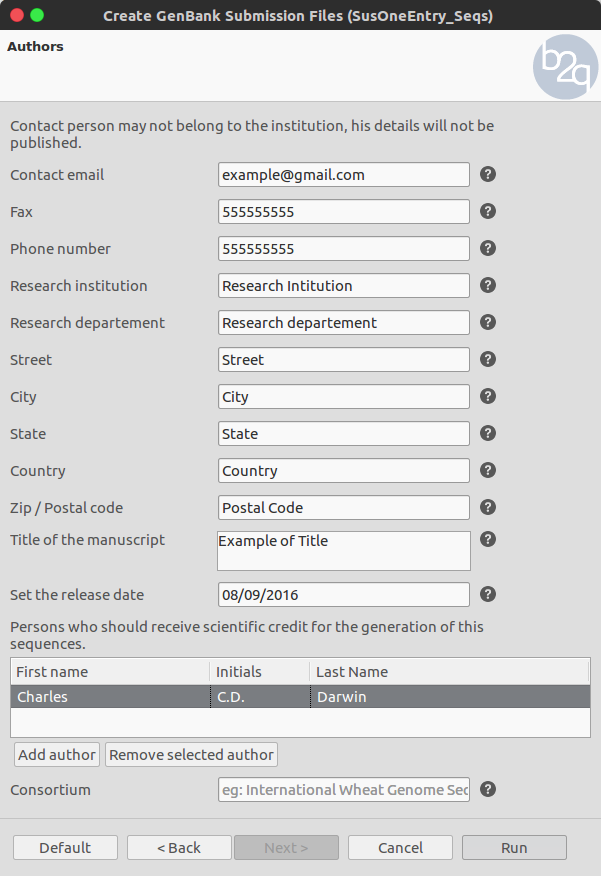
\includegraphics[width=80mm]{img/WizardPage3.png}
\caption{Author's and Affiliation page}
\label{fig:ncbisublinkfiles}
\end{figure}



\section{Results Files}
Once the input data has been analysed and processed via the tbl2asn tool, several
result files are created.
\begin{itemize}
  \item \textbf{.sqn}:This is the ASN1 file containing the compressed
information of the .tbl and .sbt files.

\item \textbf{.tbl}: The file containing the coordinates and the features
for each annotated gene.

\item \textbf{.sbt}: The file containing the authors and project
information.

  \item \textbf{.gbf}: This is the GeneBank flatfile, a previous view of the
  .sqn once it is published.

 \item \textbf{.ecn}: This file contains the Enzyme Consortium Number errors and
 the changes applied by the previous NCBI automatic validation you have just
 performed.

  \item \textbf{.val}: This is the same file as the "errorsummary.val", with
  more details and explanations, that will guide you to make the appropriate
  corrections.
   \item \textbf{.txt}: This file contains additional information about the
   errors found.
\end{itemize}

A results page provides a  a summary of the different types of errors and
warnings.
Errors must be corrected and the warnings should be reviewed (they may be
correct, depending on your data).

Modifications can be made by editing the gff or the annotation in the Blast2GO
project.
Once errors are corrected the tool can be reruned until an error-free
validattion is acheived.

Once the submission files have no errors, the ASN1 (.sqn) file is ready for submission via
the  NCBI Genomes Submission Tools
(\myurl{www.ncbi.nlm.nih.gov/projects/GenomeSubmit/genome_submit.cgi}).

Whenever you submit a new genome, it is necessary to send an email to the Submission Processing Center
(genomes@ncbi.nlm.nih.gov) specifying the registered BioProject and organism
name in the message as well as the requested release date of the genome.


\begin{figure}[!ht] \centering
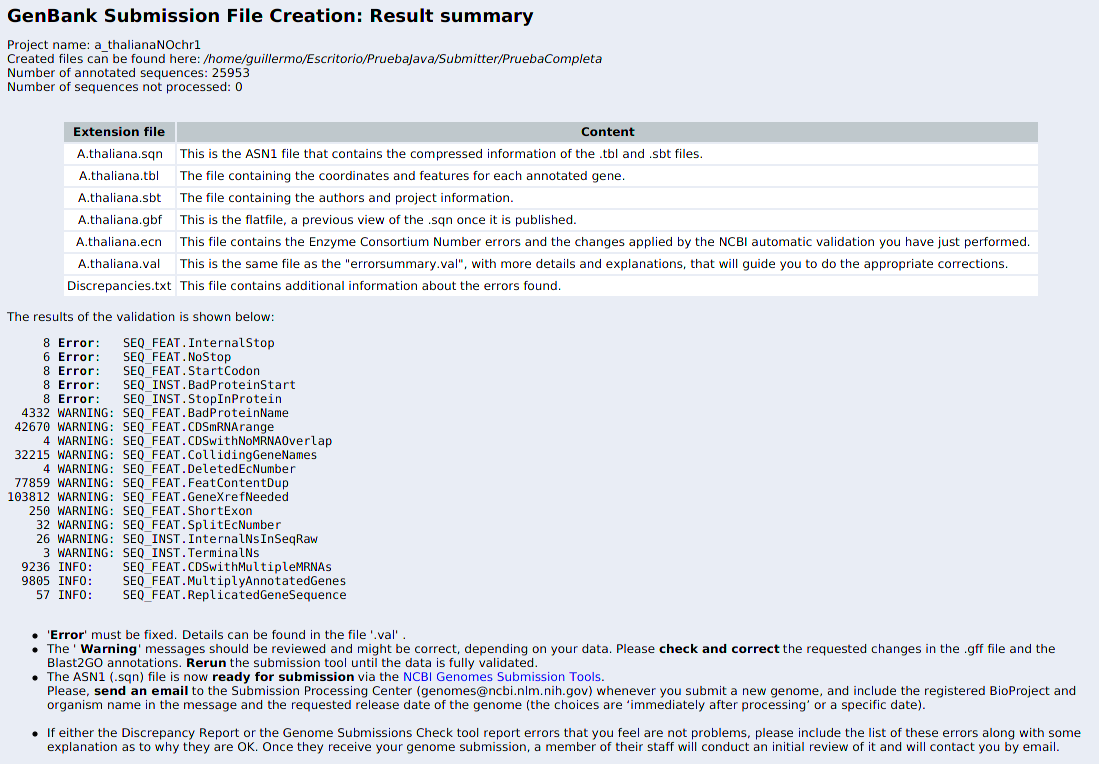
\includegraphics[width=\textwidth]{img/SummaryResults.png}
\caption{Results summary}
\label{fig:ncbisubtool}
\end{figure}

\newpage
\subsection{Most common `ERRORS' and `WARNINGS'}
\begin{itemize}
 \item \textbf{ERROR(s): InternalStop + StartCodon + BadProteinStart +
 StopInProtein}: These error codes usually appear grouped, and they refer to
 the same sequence. This may be due to an error in the gff that has shifted its
 reading frame, you can correct that by changing the frame on the .gff.
 \item \textbf{StartCodon}: An illegal start codon was used. Some possible
 explanations are: (1) the wrong genetic code may have been selected; (2)
 the wrong reading frame may be in use; or (3) the coding region may be
 incomplete at the 5' end, in which case a partial location should be indicated.
 This can be fixed in the .gff file, or by selecting the correct code in the
 `source qualifiers' on the first wizard page.
 \item \textbf{InternalStop}: Internal stop codons are found in the protein
 sequence. Some possible explanations are: (1) the wrong genetic code may have
 been selected; (2) the wrong reading frame may be in use; (3) the coding region
 may be incomplete at the 5' end, in which case a partial location should be
 indicated; or (4) the CdRegion feature location is incorrect. This can be fixed
 in the .gff file by modifying the start of the sequence or selecting the
 correct code on the `source qualifiers' on the first wizard page.
 \item \textbf{WARNING CDSmRNArange}: This error alerts you that two or more
 'CDS' features are under the same `mRNA' feature, but there are not colliding.
 If you are working with prokaryotes, this is a feature you must fix it in the
 .gff file, but if working with eukaryotes, it's a normal feature, as eukaryotic
 genes contain introns.
 \item \textbf{WARNING CDSwithNoMRNAOverlap}: This warning alerts you that
 a `CDS' feature out of the `mRNA' bounds, and should be fixed in the .gff
 file by extending the mRNA range.
 \item \textbf{WARNING BadProteinName}: The name assigned to this protein is
 not adequate. Remember that the protein name should not contain the names
 `hypothetical' or `partial', and must follow the Uni-Prot protein product
 names. Modify it in the Blast2GO project or directly in the .sqn file.
 \item \textbf{WARNING CollidingGeneNames}: Two gene features should not have
 the same name, this can be fixed in the Blast2GO project.
 \item \textbf{WARNING MissingMRNAproduct}: The mRNA feature indicates to a cDNA
 product that is not contained in the record. This must be fixed on the .gff
 file.
 \item \textbf{WARNING DuplicateInterval}: The location has identical adjacent
 intervals, e.g., a duplicate exon reference. This can be fixed eliminating the
 duplicated `exon' or `CDS' from the .gff file.
 \item \textbf{WARNING mRNAgeneRange}: An mRNA is overlapped by a gene feature,
 but is not completely contained by it. This can be corrected in the .gff by
 extending the range of the `mRNA'.
 \item \textbf{NoOrgFound}: This entry does not specify the organism that was
 the source of the sequence. Please enter a name for the organism on the first
 page of the wizard, in the `Optional source qualifiers'.
\end{itemize}

For more information about these errors, please refer to
\myurl{http://www.ncbi.nlm.nih.gov/IEB/ToolBox/C_DOC/lxr/source/errmsg/valid.msg}.







